\newcommand{\suffix}[1]{$\text{suff}_{#1}$}

\chapter{Indexeren van vaste tekst}
\begin{itemize}
    \item Sommige zoekoperaties gebeuren op een vaste tekst $T$ waarin frequent gezocht wordt naar een veranderlijk patroon $P$.
    \item Voorbereidend werk op de tekst om efficiënter te doorzoeken.
    \item Alle zoekmethoden in hoofdstuk \ref{ch:zoeken_in_strings} verrichten voorbereidend werk op het patroon.
    \begin{itemize}
        \item In het slechtste geval is dit $O(t + p)$.
        \item Dit kan gereduceerd worden tot $O(p)$ door eerst $O(t)$ voorbereidend werk te doen op $T$ via \textbf{suffixen}.
        \item Als een patroon in de tekst voorkomt, moet het een prefix zijn van één van de suffixen.
        \item Een suffix dat begint op lokatie $i$ wordt aangeduidt met \suffix{i}.
    \end{itemize}
\end{itemize}


\section{Suffixbomen}
\begin{figure}[ht]
    \centering
    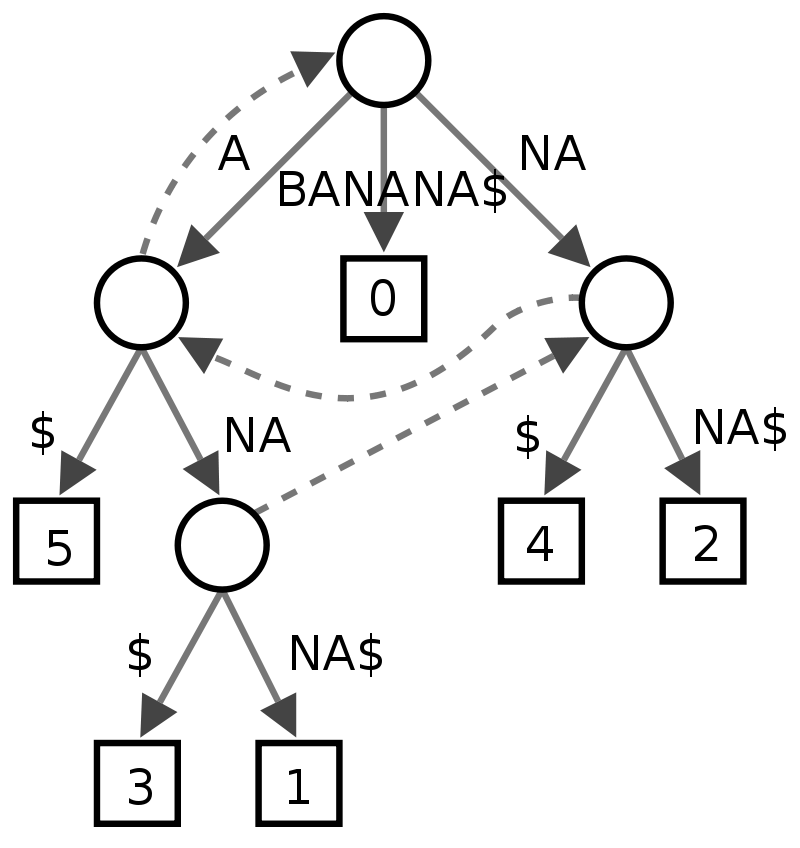
\includegraphics[width=0.3\textwidth]{suffix_tree}
    \caption{Een suffixboom voor de string \texttt{BANANA\$}. Elk van de suffixen \texttt{BANANA\$}, \texttt{ANANA\$}, \texttt{NANA\$}, \texttt{ANA\$}, \texttt{NA\$} en \texttt{A\$} kan gevonden worden in deze boom. Het suffix \texttt{NANA\$} wordt gevonden door twee keer de rechterdeelboom te nemen vanuit de wortel. De index $2$ wijst erop dat de suffix begint bij $T[2]$. De gestreepte verbindingen zijn staartpointers.}
    \label{fig:suffix_tree}
\end{figure}
\begin{itemize}
    \item Een \textbf{gewijzigde patriciatrie}:
    \begin{enumerate}
        \item In de bladeren wordt enkel de index $i$ van \suffix{i} opgeslagen, en niet het suffix zelf.
        \item In elke knoop wordt er een begin- en eindindex opgenomen, in plaats van een testindex.
        \item Elke inwendige knoop kan een staartpointer opnemen die de opbouw van de suffixboom eenvoudiger maakt.
        \begin{itemize}
            \item De staart van een string $s$ is \textbf{staart($s$)} en wordt bekomen door het eerste karakter van de string te verwijderen.
            \item De staart van een suffix is zelf ook een suffix.
        \end{itemize}
    \end{enumerate}
    \item In de trie is er een expliciete inwendige knoop horend bij de niet-lege string $\alpha$, als de trie twee strings $\alpha\beta$ en $\alpha\gamma$ bevat zodat de eerste letter van $\beta$ verschilt van de eerste letter van $\gamma$.

    \item \textbf{Twee eenvoudige toepassingen} van een suffixboom:
    \begin{enumerate}
        \item \textbf{Zoeken van een patroon $P$ in een tekst $T$.}
        \begin{itemize}
            \item Constureer de suffixboom voor $T$.
            \item Zoek de knoop die overeenkomt met $P$.
            \begin{itemize}
                \item Als deze niet bestaat zit $P$ niet in $T$.
                \item Als deze wel bestaat, zitten de gezochte beginposities in $T$ bij alle bladeren die opvolger zijn van de gevonden knoop.
            \end{itemize}
        \end{itemize}

        \item \textbf{De langste gemeenschappelijke deelstring.}
        \begin{itemize}
            \item Er is een verzameling van $k$ verschillende strings $S = \{s_1, s_2, \cdots, s_k\}$ met totale lengte $t$.
            \item De langste gemeenschappelijke deelstring van van al die strings wordt gezocht.
            \item Er wordt een \textbf{veralgemeende suffixboom} opgesteld:
            \begin{itemize}
                \item Elk blad bevat de beginpositie van het suffix, en ook tot welke strings ze behoort.
                \item Elk blad moet ook de begin- en eindindex opslagen, per eventuele string.
            \end{itemize}
            \item Elke inwendige knoop komt overeen met een prefix van een suffix, en deze deelstring komt voor in elk string die vermeld wordt bij een blad dat opvolger is van die knoop.
            \item De boom wordt overlopen om de lengte van al de prefixen en het aantal verschillende strings te bepalen waarin ze voorkomen, en dus ook het langste prefix dat in alle strings voorkomt.
        \end{itemize}
        
    \end{enumerate}
\end{itemize}

\section{Suffixtabellen}
\begin{itemize}
    \item We veronderstellen dat het vroeger gebruikte patroon $P$ (\texttt{GCAGAGCAG}) nu de tekst is, om voorbeelden in te korten.
    \item Een tabel met de gerangschikte suffixen van een string.
    \item De elementen van de tabel zijn indices, die de startpositie van het suffix aanduiden van de string.
    \begin{table}[ht]
        \centering
        \begin{tabular}{|c|ccccccccc|}
            \hline
            $i$&0&1&2&3&4&5&6&7&8\\
            $T[i]$&G&C&A&G&A&G&C&A&G\\
            \hline
            $SA[i]$&7&2&4&6&1&8&3&5&0\\
            $T[SA[i]]$&A&A&A&C&C&G&G&G&G\\
            \hline
        \end{tabular}
        \caption{De suffixtabel $SA$ voor \texttt{GCAGAGCAG}.}
        \label{table:suffixtabel}
    \end{table}
    \item Deze tabel wordt bekomen door de suffixboom in inorder te overlopen. 
    \begin{itemize}
        \item Andere, meer efficiënte, methoden bestaan, maar worden niet in de cursus besproken.
    \end{itemize}
    \item Om een suffixtabel te gebruiken is er een hulpstructuur nodig, de \textbf{LGP}-tabel (Langste Gemeenschappelijke Prefix), die dan wordt omgezet in de \textbf{LCP}-tabel die gerangschikt is in de volgorde gegeven door de suffixtabel.
    
    \item Tabel \ref{table:LCPconstruction} toont de constructie van de LCP-tabel.
    \begin{itemize}
        \item Overloop $i$, $0 \leq i \leq t$.
        \item Zoek $j$ zodanig dat $SA[j] = i$.
        \item De opvolger van $suff_i$ is dan $suff_{SA[j + 1]}$.
        \item Vergelijk $suff_i$  met $suff_{SA[j + 1]}$ vanaf beginpositie $P[i + l]$.
        \begin{itemize}
            \item Initieel is $l = 0$.
            \item Verhoog $l$ totdat $T[i + l] \neq T[SA[j + 1] + l]$.
            \item Als $l > 0$, dan moet voor $i + 1$ slechts vergeleken worden vanaf $T[i + l - 1]$.
        \end{itemize}
    \end{itemize}
    
    
    \begin{table}[ht]
        \centering
        \begin{tabular}{|ccc|c|ccccccccc|}
            \hline
            &&&$i$&0&1&2&3&4&5&6&7&8\\
            &&&$T[i]$&G&C&A&G&A&G&C&A&G\\
            \hline
            &&&$SA[i]$&7&2&4&6&1&8&3&5&0\\
            &&&$T[SA[i]]$&A&A&A&C&C&G&G&G&G\\
            \hline
            \textbf{i}&\textbf{opvolger}&\textbf{LGP[i]}&l&0&1&2&3&4&5&6&7&8\\
            \hdashline
    
            0&-&0&$/$&&&&&&&&&\\
            \hdashline
            1&8&0&$suff_1$&\nm{C}&A&G&A&G&C&A&G&\\
             & & &$suff_8$&\nm{G}&&&&&&&& \\
             \hdashline
    
            2&4&2&$suff_2$&\m{A}&\m{G}&\nm{A}&G&C&A&G&&\\
            & & &$suff_4$&\m{A}&\m{G}&\nm{C}&A&G&&&& \\
            \hdashline
    
            3&5&1&$suff_3$&\um{G}&\nm{A}&G&C&A&G&&&  \\
             & & &$suff_5$&\um{G}&\nm{C}&A&G&&&&& \\
             \hdashline
    
            4&6&0&$suff_4$&\nm{A}&G&C&A&G&&&&  \\
             & & &$suff_6$&\nm{C}&A&G&&&&&&\\
             \hdashline
    
            5&0&4&$suff_5$&\m{G}&\m{C}&\m{A}&\m{G}&&&&& \\
             & & &$suff_0$&\m{G}&\m{C}&\m{A}&\m{G}&A&G&C&A&G \\
             \hdashline
            6&1&3&$suff_6$&\um{C}&\um{A}&\um{G}&&&&&& \\
             & & &$suff_1$&\um{C}&\um{A}&\um{G}&A&G&C&A&G& \\
             \hdashline
            
            7&2&2&$suff_7$&\um{A}&\um{G}&&&&&&& \\
             & & &$suff_2$&\um{A}&\um{G}&A&G&C&A&G&& \\
             \hdashline
            8&3&1&$suff_8$&\um{G}&&&&&&&& \\
             & & &$suff_3$&\um{G}&A&G&C&A&G&&& \\
            \hline
             & & & $LGP[i]$&0&0&2&1&0&4&3&2&1\\
             & & & $LCP[i]$&4&0&0&1&2&0&3&1&2\\
             \hline
        \end{tabular}
        \caption{De constructie van de LCP-tabel voor \texttt{GCAGAGCAG}. Karakters die rood of groen zijn worden effectief vergeleken. Oranje karakters moeten niet meer vergeleken worden.}
        \label{table:LCPconstruction}
    \end{table}


    \item Een patroon $P$ opzoeken in de suffixtabel gebeurt met \textbf{binair zoeken}.
\end{itemize}

\section{Tekstzoekmachines}
\subsection{Inleiding}
\begin{itemize}
    \item Tekstzoekmachines zijn in eerste instantie gelijkaardig aan databanksystemen.
    \begin{itemize}
        \item Documenten worden bewaard in een repository.
        \item Er worden indexen bijgehouden om snel documenten te doorlopen.
        \item Er kunnen queries uitgevoerd worden relevante documenten te zoeken.
    \end{itemize}
    \item Maar ze verschillen ook van databanksystemen.
    \begin{itemize}
        \item Een query voor een tekstzoekmachine bestaat enkel uit woorden of zinnen.
        \item In een databanksysteem zal de query resultaten geven die voldoen aan een logische uitspraak, maar bij een tekstzoekmachine is dit vager.
        \item Een tekstzoekmachine geeft niet alle resultaten terug, maar enkel de meest relevante. Het begrip relevantie is ook niet exact, aangezien dit afhangt van de gebruiker.
    \end{itemize}
    \item Het gebruik van \textbf{indices} om tekst te indexeren is onmisbaar.
\end{itemize}

\subsection{Zoeken van tekst en informatie verzamelen}
\subsubsection{Queries}
\begin{itemize}
    \item In een traditionele databank hebben gegevens een unieke sleutel, wat niet het geval is bij tekstdocumenten op het internet.
    \item Soms hebben tekstdocumenten \textit{metadata} zoals de auteur, het onderwerp en het aantal pagina's, maar deze zijn slechts occasioneel nuttig.
    \item De meest voorkomende manier om in tekst te zoeken is het zoeken naar \textbf{inhoud} aan de hand van een \textbf{query}.
    \item Aangezien dat een tekstzoekmachine probeert relevante documenten weer te geven, moet gemeten kunnen worden hoe goed deze documenten zijn.
    \item Een tekstzoekmachine heeft een bepaalde \textbf{effectiveness} voor een getal $r$ waarbij de meeste van de eerste $r$ resultaten relevant zijn. 
    \begin{itemize}
        \item De \textit{effectiveness} wordt vaak bepaald door de \textbf{precision} en \textbf{recall}.
        \item De \textit{precision} is de verhouding van documenten  dat relevant zijn.
        \item De \textit{recall} is de verhouding van relevante documenten die gekozen zijn.
        \item Voorbeeld:
        \begin{itemize}
            \item Een tekstdatabank bevat 20 documenten.
            \item Een gebruiker zoekt in deze databank met een query en er worden 8 resultaten teruggegeven.
            \item De gebruiker vindt dat 5 van deze resultaten relevant zijn voor hem, en dat er nog 2 andere documenten in de tekstdatabank zitten die niet door de tekstzoekmachine gegeven worden.
            \item De textit{precision} is $5/8$.
            \item De \textit{recall} is $5/7$.
        \end{itemize}
        \item Veel van de technieken zorgen ervoor dat \textit{effectiveness} vrij hoog blijft.
    \end{itemize}
\end{itemize}
\subsubsection{Voorbeelddatabanken}
\begin{itemize}
    \item De \textbf{Keeper databank}.
    \begin{align*}
        1\qquad& \hbox{The old night keeper keeps the keep in the town.}\\
        2\qquad& \hbox{In the big old house in the bog old gown.}\\
        3\qquad& \hbox{The house in the town had the big old keep.}\\
        4\qquad& \hbox{Where the old night keeper never did sleep.}\\
        5\qquad& \hbox{The night keeper keeps the keep in the night.}\\
        6\qquad& \hbox{And keeps in the dark and sleeps in the night.}\\
    \end{align*}

    \begin{itemize}
        \item Bevat 6 documenten elk met 1 lijn.

        \item Verschillende eenvoudige technieken om in deze databank te zoeken.
        \begin{itemize}
            \item De query \texttt{big old house} waarbij de query als één enkele string beschouwd wordt zal enkel document 2 geven.
            \item De query \texttt{big old house} waarbij elk woord in een verzameling van woorden komt (\textbf{bag-of-word}, \{\texttt{big}, \texttt{old}, \texttt{house}\}) zal documenten 2 en 3 teruggeven. De volgorde van de woorden in deze verzameling spelen geen rol en elk woord wordt afzonderlijk bekeken of ze voorkomt in het document of niet.
        \end{itemize}
        \item Meerdere technieken om de \textbf{woordenschat} van een tekstdatabank te reduceren:
        \begin{itemize}
            \item \textbf{Zonder aanpassingen}

            \texttt{And and big dark did gown had house In in keep keeper keeps light never night old sleep sleeps The the town Where}
            \item \textbf{Hoofdletter-invariantie}

            \texttt{and big dark did gown had house in keep keeper keeps light never night old sleep sleeps the town where}

            \item \textbf{Verwijderen meerdere varianten van hetzelfde woord}

            \texttt{and big dark did gown had house in keep light never night old sleep the town where}

            \item \textbf{Verwijderen van vaak voorkomende woorden}

            \texttt{big dark did gown house keep light night old sleep town}
        \end{itemize}
    \end{itemize}

    \item Twee hypothetische databanken om efficiëntie te bespreken:
    \begin{table}[ht]
        \centering
        \begin{tabular}{l r r}
            \hline
            & NewsWire & Web \\
            \hline
            Grootte in gigabytes & 1 & 100 \\
            Aantal Documenten & 400 000 & 12 000 000 \\
            Aantal woorden   & 180 000 000 & 11 000 000 000 \\
            Aantal unieke woorden & 400 000 & 16 000 000 \\
            Aantal unieke woorden per document, opgesomd & 70 000 000 & 3 500 000 000 \\
            \hline
        \end{tabular}
    \end{table}
    \item Elke tekstzoekmachine moet aan een aantal voorwaarden voldoen:
    \begin{itemize}
        \item De queries moeten goed geanalyseerd worden.
        \item De queries moeten snel geanalyseerd worden.
        \item Minimaal gebruik van resources zoals geheugen en bandbreedte.
        \item Schaalbaar naar grote volumes van data.
        \item Resistent tegen het wijzigen van documenten.
    \end{itemize}
\end{itemize}

\subsubsection{Gelijkaardigheidsfuncties}
\begin{itemize}
    \item Elke tekstzoekmachine maakt gebruik van een rankingsysteem om documenten te ordenen.
    \item Om documenten te ordenen wordt er gebruik gemaakt van een gelijkaardigheidsfunctie.
    \item Hoe hoger de waarde van deze functie, hoe hoger de kans dat de gebruiker dit document als relevant zal beschouwen.
    \item De $r$ meest relevante documenten worden dan gegeven aan de gebruiker.
    \item In \textbf{bag-of-words} queries wordt de gelijkaardigheidsfunctie samengesteld door een aantal statistische variabelen:
    \begin{itemize}
        \item $f_{d, t}$ is de frequentie van het woord $t$ in document $d$.
        \item $f_{q, t}$ is de frequentie van het woord $t$ in de query $q$.
        \item $f_t$ is het aantal documenten dat één of meer keer het woord $t$ bevat.
        \item $F_t$ is het aantal keer dat $t$ voorkomt in de hele tekstdatabank.
        \item $N$ is het aantal documenten in de tekstdatabank.
        \item $n$ het aantal geïndexeerde woorden in de tekstdatabank.
    \end{itemize}
    \item Deze waarden kunnen gecombineerd worden om drie vaststellingen te maken:
    \begin{enumerate}
        \item Een woord dat in veel documenten voorkomt krijgt een kleiner gewicht.
        \item Een woord dat veel in één document voorkomt krijgt een groter gewicht.
        \item Een document dat veel woorden bevat krijgt een kleiner gewicht. 
    \end{enumerate}
    \item Er is een \textbf{query vector $\vec{w}_q$} en een \textbf{document vector $\vec{w}_d$}, waarbij elk component in deze vector gedefinieerd wordt als
    $$w_{q, t} = \ln\bigg( \frac{N}{f_t}\bigg) \qquad w_{d, t} = f_{d,t}$$
    \item De maat van gelijkheid $S_{q, d}$, de maat in hoeverre het document $d$ relevant is voor query $q$, kan bekomen worden door de cosinus van de hoek tussen deze twee vectoren te nemen.
    $$S_{q, d} = \frac{\vec{w}_d \cdot \vec{w}_q}{||\vec{w}_d||\cdot ||\vec{w}_q||} = \frac{\sum_t w_{d,t} \cdot w_{q,t}}{\sqrt{\sum_t w^2_{d,t}}\cdot \sqrt{\sum_t w^2_{q,t}}}$$
    \item De grootheid $w_{q, t}$ encodeert de \textbf{inverse document frequentie} van een woord $t$.
    \item De grootheid $w_{d, t}$ encodeert de \textbf{woord frequentie} van een woord $t$.
    \item Het nadeel aan deze methode is dat elk document in beschouwing genomen moet worden, maar dat slechts $r$ documenten gevonden moeten worden.
    \item Voor de meeste documenten is de gelijkaardigheidswaarden insignificant.
    \item Deze \textbf{brute-force} methode kan uitgebreidt worden tot betere methoden, via \textbf{indices}.
\end{itemize}


\subsection{Indexeren en query-evaluatie}
\begin{itemize}
    \item Een \textbf{index} in deze context is een datastructuur dat een woord afbeeldt op documenten dat dit woord bevat.
    \item Het verwerken van een query kan dan enkel uitgevoerd worden op documenten die minstens één van de query woorden bevat.
    \item Er zijn vele soorten indices, maar de meest gebruikte is een \textbf{inverted file index}: een collectie van lijsten, één per woord, dat documenten bevat dat dit woord bevat.

    \item Een \textbf{normale inverted file index} bestaat uit twee componenten. 
    \begin{enumerate}
        \item Voor elk woord $t$ houdt de \textbf{zoekstructuur} het volgende bij:
        \begin{itemize}
            \item een getal $f_t$ van het aantal documenten dat $t$ bevat, en 
            \item een pointer naar de start van de correspondeerde geïnverteerde lijst.
        \end{itemize}
        \item Een \textbf{verzameling van geïnverteerde lijsten}, waarbij elk lijst het volgende bijhoudt voor een woord $t$:
        \begin{itemize}
            \item de sleutels van documenten $d$ die $t$ bevatten, en 
            \item de verzameling van frequencies $f_{d,t}$ van woorden $t$ in document $d$.
            \item $\rightarrow \langle d, f_{d,t}\rangle$ paren.
        \end{itemize}
    \end{enumerate}
    \item Samen met $W_{d}$ en deze twee componenten zijn geordende queries mogelijk.
    \item Een \textit{inverted file} voor de \textit{keeper database} is te zien op tabel \ref{table:inverted_file_keeper}.


    \begin{table}[ht]
        \centering
        \begin{tabular}{l c | l}
            woord $t$ & $f_t$ & Geïnverteerde lijst voor $t$ \\
            \hline
            \texttt{and}    & 1 & $\langle 6, 2\rangle$ \\
            \texttt{big}    & 2 & $\langle 2, 2\rangle\ \langle 3, 1\rangle$\\
            \texttt{dark}   & 1 & $\langle 6, 1\rangle$\\
            \texttt{did}    & 1 & $\langle 4, 1\rangle$\\
            \texttt{gown}   & 1 & $\langle 2, 1\rangle$\\
            \texttt{had}    & 1 & $\langle 3, 1\rangle$\\
            \texttt{house}  & 2 & $\langle 2, 1\rangle\ \langle 3, 1\rangle$\\
            \texttt{in}     & 5 & $\langle 1, 1\rangle\ \langle 2, 2\rangle\ \langle 3, 1\rangle\ \langle 5, 1\rangle\ \langle 6, 2\rangle$\\
            \texttt{keep}   & 3 & $\langle 1, 1\rangle\ \langle 3, 1\rangle\ \langle 5, 1\rangle$\\
            \texttt{keeper} & 3 & $\langle 1, 1\rangle\ \langle 4, 1\rangle\ \langle 5, 1\rangle$\\
            \texttt{keeps}  & 3 & $\langle 1, 1\rangle\ \langle 5, 1\rangle\ \langle 6, 1\rangle$\\
            \texttt{light}  & 1 & $\langle 6, 1\rangle$\\
            \texttt{never}  & 1 & $\langle 4, 1\rangle$\\
            \texttt{night}  & 3 & $\langle 1, 1\rangle\ \langle 4, 1\rangle\ \langle 5, 1\rangle$\\
            \texttt{old}    & 4 & $\langle 1, 1\rangle\ \langle 2, 2\rangle\ \langle 3, 1\rangle\ \langle 4, 1\rangle$\\
            \texttt{sleep}  & 1 & $\langle 4, 1\rangle$\\
            \texttt{sleeps} & 1 & $\langle 6, 1\rangle$\\
            \texttt{the}    & 6 & $\langle 1, 3\rangle\ \langle 2, 2\rangle\ \langle 3, 3\rangle\ \langle 4, 1\rangle\ \langle 5, 3\rangle\ \langle 6, 2\rangle$\\
            \texttt{town}   & 2 & $\langle 1, 1\rangle\ \langle 3, 1\rangle$\\
            \texttt{where}  & 1 & $\langle 4, 1\rangle$\\
        \end{tabular}
        \begin{tabular}{c |c c c c c c}
            $d$ & 1 & 2 & 3 & 4 & 5 & 6\\
            \hline
            $W_d$ & 4 & 4.2 & 4 & 2.8 & 4.1 & 4

        \end{tabular}
        \caption{Een op document niveau geïnverteerd bestand voor de \textit{Keeper} databank. Elk woord $t$ bestaat uit $f_t$ en een lijst van paren, waarbij elk paar bestaat uit een sleutel $d$ van een document en de frequentie $f_{d, t}$ van het woord $t$ in $d$. Ook zijn de waarden van $W_d$ te zien, berekend volgens $W_d = \sqrt{\sum_t w^2_{d, t}} = \sqrt{\sum_t f^2_{d, t}}$.}
        \label{table:inverted_file_keeper}
    \end{table}
    \item Er kan nu een \textbf{query evaluatie} algoritme opgesteld worden (gevisualiseerd op figuur \ref{fig:inverted_files_similarity_scores}).
    \begin{figure}[ht]
        \centering
        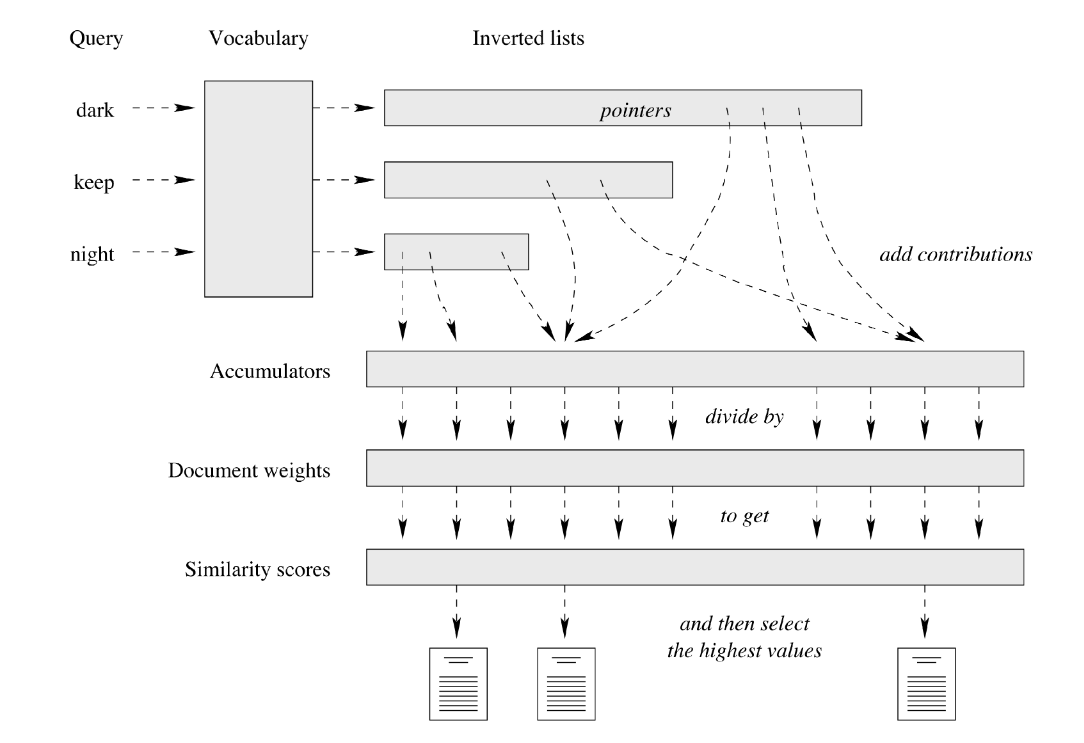
\includegraphics[width=0.7\textwidth]{inverted_files_similarity_scores}
        \caption{Het gebruik van een geïnverteerd bestand en een verzameling van accumulators om gelijkaardigheidswaarden te berekenen.}
        \label{fig:inverted_files_similarity_scores}
    \end{figure}
    \begin{enumerate}
        \item Er wordt een accumulator $A_d$ bijgehouden voor elk document $d$. Initieel is elke $A_d = 0$.
        \item Voor elk woord $t$ in de query worden volgende operaties uitgevoerd:
        \begin{enumerate}
            \item Bereken $w_{q, t} = \ln\bigg(\frac{N}{f_t}\bigg)$ en vraag de geïnverteerde lijst op van $t$.
            \item Voor elk paar $\langle d, f_{d,t} \rangle$ in de geïnverteerde lijst worden volgende operaties uitgevoerd:
            \begin{enumerate}
                \item Bereken $w_{d, t}$.
                \item Stel  $A_d = A_d + w_{q,t}w_{d,t}$.
            \end{enumerate}
        \end{enumerate}
        \item Voor elke $A_d > 0$, stel $S_d = A_d/W_d$.
        \item Identificeer de $r$ grootste $S_d$ waarden en geef de correspondeerde documenten terug.
    \end{enumerate}
    
    \item Het is ook nog mogelijk om \textbf{de posities van de woorden in het document te indexeren}.
    \begin{itemize}
        \item Het paar $\langle d, f_{d,t}\rangle$ kan uitgebreidt worden om de posities $p$ bij te houden waar dat $t$ voorkomt in $d$.
        $$\langle d, f_{d, t}, p_1, \cdots, p_{f_{d,t}}\rangle$$
    \end{itemize}
\end{itemize}

\subsection{Queries met zinnen}
\begin{itemize}
    \item Een query kan een expliciete zin bevatten, aangeduid met aanhalingstekens, zoals \texttt{"philip glass"} of \texttt{"the great flydini"}.
    \item Soms is het ook impliciet zoals \texttt{Albert Einstein} of \texttt{San Francisco hotel}.
    \item \todo{idk}
\end{itemize}

\subsection{Constructie van een index}
\begin{itemize}
    \item Het volume van de data is veel te groot om alles in het geheugen te doen.
    \item Er zijn drie methoden:
    \begin{enumerate}
        \item \textbf{In-memory Inversion}
        \begin{itemize}
            \item Alle documenten wordt tweemaal overlopen.
            \begin{enumerate}
                \item Een eerste keer telt de frequentie $f_t$ van alle verschillende woorden van alle documenten.
                \item Een tweede maal plaatst de pointers in de juiste positie.
            \end{enumerate}
        \end{itemize}

        \item \textbf{Sort-Based Inversion}

        \item \textbf{Merge-Based Inversion}
    \end{enumerate}
\end{itemize}